%% abtex2-modelo-artigo.tex, v-1.9.6 laurocesar
%% Copyright 2012-2016 by abnTeX2 group at http://www.abntex.net.br/ 
%%
%% This work may be distributed and/or modified under the
%% conditions of the LaTeX Project Public License, either version 1.3
%% of this license or (at your option) any later version.
%% The latest version of this license is in
%%   http://www.latex-project.org/lppl.txt
%% and version 1.3 or later is part of all distributions of LaTeX
%% version 2005/12/01 or later.
%%
%% This work has the LPPL maintenance status `maintained'.
%% 
%% The Current Maintainer of this work is the abnTeX2 team, led
%% by Lauro César Araujo. Further information are available on 
%% http://www.abntex.net.br/
%%
%% This work consists of the files abntex2-modelo-artigo.tex and
%% abntex2-modelo-references.bib
%%

% ------------------------------------------------------------------------
% ------------------------------------------------------------------------
% abnTeX2: Modelo de Artigo Acadêmico em conformidade com
% ABNT NBR 6022:2003: Informação e documentação - Artigo em publicação 
% periódica científica impressa - Apresentação
% ------------------------------------------------------------------------
% ------------------------------------------------------------------------

\documentclass[
	% -- opções da classe memoir --
	article,			% indica que é um artigo acadêmico
	11pt,				% tamanho da fonte
	oneside,			% para impressão apenas no recto. Oposto a twoside
	a4paper,			% tamanho do papel. 
%  twocolumn
	% -- opções da classe abntex2 --
	%chapter=TITLE,		% títulos de capítulos convertidos em letras maiúsculas
	%section=TITLE,		% títulos de seções convertidos em letras maiúsculas
	%subsection=TITLE,	% títulos de subseções convertidos em letras maiúsculas
	%subsubsection=TITLE % títulos de subsubseções convertidos em letras maiúsculas
	% -- opções do pacote babel --
	english,			% idioma adicional para hifenização
	brazil,				% o último idioma é o principal do documento
	sumario=tradicional
	]{abntex2}


% ---
% PACOTES
% ---

% ---
% Pacotes fundamentais 
% ---
\usepackage{lmodern}			% Usa a fonte Latin Modern
\usepackage[T1]{fontenc}		% Selecao de codigos de fonte.
\usepackage[utf8]{inputenc}		% Codificacao do documento (conversão automática dos acentos)
\usepackage{indentfirst}		% Indenta o primeiro parágrafo de cada seção.
\usepackage{nomencl} 			% Lista de simbolos
\usepackage{color}				% Controle das cores
\usepackage{graphicx}			% Inclusão de gráficos
\usepackage{microtype} 			% para melhorias de justificação
% ---
		
% ---
% Pacotes adicionais, usados apenas no âmbito do Modelo Canônico do abnteX2
% ---
\usepackage{lipsum}				% para geração de dummy text
% ---

\graphicspath{{figuras/}}

\usepackage{float}
\usepackage{amsmath}
\usepackage{amsfonts}
\usepackage{amssymb}
\usepackage{multirow,tabularx}
\usepackage{multicol}

% ---
% Pacotes de citações
% ---
\usepackage[brazilian,hyperpageref]{backref}	 % Paginas com as citações na bibl
\usepackage[alf]{abntex2cite}	% Citações padrão ABNT
% ---

% ---
% Configurações do pacote backref
% Usado sem a opção hyperpageref de backref
\renewcommand{\backrefpagesname}{Citado na(s) página(s):~}
% Texto padrão antes do número das páginas
\renewcommand{\backref}{}
% Define os textos da citação
\renewcommand*{\backrefalt}[4]{
	\ifcase #1 %
		Nenhuma citação no texto.%
	\or
		Citado na página #2.%
	\else
		Citado #1 vezes nas páginas #2.%
	\fi}%
% ---

%\renewcommand{\thesection}{\Roman{section}} 
%\renewcommand{\thesubsection}{\Alph{subsection}}

% ---
% Informações de dados para CAPA e FOLHA DE ROSTO
% ---
\titulo{\textbf{Sistema de Irrigação Fuzzy}}
\autor{
    \textbf{Erick Alves Augusto}\\
    {\small Centro de Matemática, Computação e Cognição}\\
    {\small Universidade Federal do ABC}\\
    {\small Santo André - SP, Brasil}\\
    {\small \texttt{erick.augusto@aluno.ufabc.edu.br}}
  \and
    \textbf{Rafael Cardoso da Silva}\\
    {\small Centro de Matemática, Computação e Cognição}\\
    {\small Universidade Federal do ABC}\\
    {\small Santo André - SP, Brasil}\\
    {\small \texttt{rafael.cardoso@aluno.ufabc.edu.br}}
}
\local{Santo André - SP, Brasil}
\data{1 de dezembro de 2016}
% ---

% ---
% Configurações de aparência do PDF final

% alterando o aspecto da cor azul
\definecolor{blue}{RGB}{41,5,195}

% informações do PDF
\makeatletter
\hypersetup{
  %pagebackref=true,
  pdftitle={Sistema de Irrigação Fuzzy}, 
  pdfauthor={Erick Alves Augusto e Rafael Cardoso da Silva},
  pdfsubject={UFABC},
  pdfcreator={LaTeX with abnTeX2},
  pdfkeywords={Sistema Fuzzy}{Controle de Irrigação}{Sistema Automatizado}, 
  colorlinks=true,       		% false: boxed links; true: colored links
  linkcolor=blue,          	% color of internal links
  citecolor=blue,        		% color of links to bibliography
  filecolor=magenta,      	% color of file links
  urlcolor=blue,
  bookmarksdepth=4
}
\makeatother
% --- 

% ---
% compila o indice
% ---
\makeindex
% ---

% ---
% Altera as margens padrões
% ---
\setlrmarginsandblock{1.3cm}{1.3cm}{*}
\setulmarginsandblock{2cm}{2cm}{*}
\checkandfixthelayout
% ---

% --- 
% Espaçamentos entre linhas e parágrafos 
% --- 

% O tamanho do parágrafo é dado por:
\setlength{\parindent}{1.3cm}

% Controle do espaçamento entre um parágrafo e outro:
\setlength{\parskip}{0.2cm}  % tente também \onelineskip

% Espaçamento simples
\SingleSpacing

% ----
% Início do documento
% ----
\begin{document}

% Seleciona o idioma do documento (conforme pacotes do babel)
%\selectlanguage{english}
\selectlanguage{brazil}

% Retira espaço extra obsoleto entre as frases.
\frenchspacing 

% ----------------------------------------------------------
% ELEMENTOS PRÉ-TEXTUAIS
% ----------------------------------------------------------
%

%---
%
% Se desejar escrever o artigo em duas colunas, descomente a linha abaixo
% e a linha com o texto ``FIM DE ARTIGO EM DUAS COLUNAS''.
% \twocolumn[    		% INICIO DE ARTIGO EM DUAS COLUNAS
%---
% página de titulo
\maketitle


% resumo em português
\begin{resumoumacoluna}
{\large 
  Muitos sistemas costumam ser automatizados, porém esses sistemas não tem a capacidade de tomar decisões em situações intermediárias. Um sistema fuzzy tem a capacidade de lidar com essas situações. Este trabalho visa testar a eficiência de um sistema fuzzy para controlar o tempo de irrigação de uma plantação. E baseado em modelos já bem estudados, em outros trabalhos já publicados, realizamos a implementação deste modelo utilizando Lógica Fuzzy. Por meio dos resultados será possível verificar se um sistema fuzzy pode ser usado no lugar de um sistema automatizado padrão.
  
 \noindent
 \textbf{Palavras-chave}: Sistema Fuzzy, Controle de Irrigação, Sistema Automatizado.

 \vspace{\onelineskip}
} 
\end{resumoumacoluna}

% ]  				% FIM DE ARTIGO EM DUAS COLUNAS
% ---

% ----------------------------------------------------------
% ELEMENTOS TEXTUAIS
% ----------------------------------------------------------
\textual

% ----------------------------------------------------------
% Introdução
% ----------------------------------------------------------

\begin{multicols}{2}
\section{Introdução}

Agricultores sempre estão preocupados com os cuidados que suas lavouras precisam. Entre as coisas que mais os preocupam é o gerenciamento de água para as plantações.

A água é um recurso essencial para o cultivo de qualquer tipo de plantação, então os agricultores tentam estar regando as suas plantações sempre que necessário, mas nem sempre a água é usada de forma correta para realizar a irrigação. Por isso foi pensado em se criar um sistema que fosse capaz de automatizar esse trabalho, mas de forma diferente dos sistemas comuns que fazem esses serviço. Existem muitos sistemas automatizados de irrigação, mas eles apenas usam períodos de irrigação definidos e não o que as plantas precisam a cada momento, por isso foi decidido criar esse sistema utilizando a lógica fuzzy.

O principal problema é descobrir a quantidade de água ideal para se irrigar a plantação a cada momento. A quantidade de água que a plantação precisa em um dia com a temperatura de 30º C não é a mesma que a plantação precisa em um dia com 20º C. Então como descobrir a quantidade certa de água para irrigar a plantação a cada momento?

É necessário descobrir quais fatores estão envolvidos para se determinar a quantidade certa de água, então é necessário coletar dados sobre a temperatura, umidade do solo e o desenvolvimento da plantação. Usando esses fatores deve ser possível chegar a um valor adequado para a quantidade de água que deve ser usada. Essa quantidade será determinada pelo tempo de irrigação, que será o tempo necessário para que a umidade do solo chegue perto de 100\%, fornecendo a quantidade ideal de água para a plantação.

Outros trabalhos desenvolvidos usando lógica fuzzy para controlar a irrigação do solo usaram outros fatores como a radiação e a salinidade do solo, além de outras formas de modelagem. Esses trabalhos fornecem uma base para saber como usar as informações para determinar o conjunto de regras que irá ajudar a indicar a quantidade de tempo necessário para a irrigação umedecer o solo na quantidade que ele precisa.

Um desses trabalhos modelou o sistema para uma plantação de pimenta no México, o conjunto de regras apresentado é completo, mas apenas para um determinado estágio do crescimento da plantação. Este trabalho usa como entrada a temperatura, umidade do solo e o estágio de crescimento da plantação. A saída retornada é o tempo de irrigação.

O trabalho foi desenvolvido usando a biblioteca JFuzzyLogic disponível para a linguagem JAVA. Por meio dela é possível fazer o processo de fuzzificação das variáveis de entrada, aplicar as regras nos valores fuzzificados, realizar a agregação dos resultados e defuzzificar para um valor exato o resultado da agregação. Essa biblioteca foi usada por fornecer todos os procedimentos necessários para o processo que deve ser realizado na lógica fuzzy.

Os resultados mostram valores de tempo para irrigar uma determinada plantação durante os três estágios definidos de desenvolvimento, esses valores podem ser usados como base para poder modelar sistemas especializados na irrigação de outros meios de cultura, sendo necessário apenas modelar os estágios de crescimento da mesma.

O trabalho possui seções que apresentam os conceitos de lógica fuzzy, a apresentação dos trabalhos que serviram de base para o projeto, a modelagem do sistema, as variáveis linguísticas e seus conjuntos fuzzy, a base de regras e os cenários testados.


\section{Lógica Fuzzy: Conceitos Fundamentais}

Nas seções seguintes serão apresentado os conceito referentes a Lógica Fuzzy, este conteúdo é explanado pelos autores~\cite{mortari2001introduccao},~\cite{hung2006first} e~\cite{rezende2003sistemas}.


A teoria clássica de conjuntos permite o tratamento de classes de objetos e suas interrelações em um universo definido. Nessa teoria, a pertinência de um dado elemento com relação a um conjunto refere-se ao fato de tal elemento pertencer ou não a esse conjunto. Por exemplo, um pessoa que tenha 20 anos, ela pode ser considerada jovem ou adulta, mas nunca os dois. Forçando assim a uma separação de membros dos não membros de uma classe, e isto pode ser um processo complicado, que muitas vezes não reflete a realidade do problema.

Já a Lógica Fuzzy utiliza a idéia de que todas as coisas admitem graus de pertinências. Assim, um elemento pertence a um conjunto com um certo grau de pertinência, fazendo com que uma determinada sentença possa ser parcialmente verdadeira e parcialmente falsa. Além do mais, um mesmo elemento pode ter graus de pertinências diferentes de 0 para mais de um conjunto fuzzy. 
O termo fuzzy em inglês tem vários significadas, sua traduções mais comuns são “nebuloso” e “difuso”.

Ainda considerando o exemplo anterior, a idade de uma pessoa pode ser descrita em conjuntos fuzzy. Na Lógica Fuzzy, não existe um limite abrupto que define os elementos que pertencem ou não a um determinado conjunto, como no caso dos conjuntos jovem e adulto. Por outro lado, os graus de pertinência dos elementos possuem variações suaves no intervalo real [0,1], representando, assim, de forma mais realista, o conhecimento humano. 

A lógica fuzzy, retrata o jeito como as pessoas pensam, modelando a sua percepção em relação às palavras, tomadas de decisões ou senso comum. Em decorrência disto, a introdução da Lógica Fuzzy tem conduzido as pesquisas para o modelamento computacional de sistemas inteligentes com raciocínios mais humanos, que é impreciso, ambíguo e vago, porém mais adequado a realidade. Ela é uma ferramenta capaz de capturar informações vagas, em geral, descritas em linguagem natural e convertê-las para um formato numérico, de fácil manipulação.


\subsection{Conceitos de Lógica Fuzzy}

A Lógica Fuzzy é baseada na ideia de informação possibilista, ou seja, uma informação que possui incerteza com respeito ao seu valor verdade.

Ela modela variáveis que podem assumir diferentes valores de acordo com a situação e ponto de vista, isso permite que essas variáveis sejam mais flexíveis e sejam capazes de se aproximar dos valores que uma pessoa poderia atribuir a cada variável devido a sua experiência.

Um valor numérico pode ser associado a uma variável linguística por meio de uma função de pertinência. Para cada conjunto é criada uma função para determinar o valor de pertinência para o elemento dentro de seu domínio, com saída que será entre 0 e 1. Assim, esta função determinará o grau de pertinência que um valor qualquer pertence aquele conjunto.

As funções podem ser representadas por funções várias funções de uma variável, dentre elas estão as Triangulares e Trapezoidais, por exemplo.

A Função Triangular é uma função que possui simetria ímpar. Ela segue uma função linear crescente e após atingir o valor máximo ela decresce com a mesma velocidade que cresceu. Já a Função Trapezoidal apresenta um crescimento baseado em uma função linear até atingir um determinado limiar, depois assume um valor constante neste limiar e, por fim, decresce.


\subsection{Sistema de Inferência Fuzzy}

O sistema de inferência usado em lógica fuzzy precisa receber as variáveis modeladas para conjuntos fuzzy, somente depois disso ele será capaz de processá-las.

Para que as variáveis de entrada e saída sejam passadas para valores fuzzy é preciso primeiro fazer a definição delas como variáveis linguísticas. Isso ocorre na interface de fuzzificação.

As variáveis de entrada recebem os dados que serão usados pelo sistema para fazer o processamento da informação e gerar a variável de saída, que é o conhecimento adquirido por meio da entrada, então os valores exatos dessas variáveis são passados para conjuntos que sejam capazes de representar os possíveis valores que essas variáveis possam assumir. Esses conjuntos são os conjuntos fuzzy.

A cada variável linguística podem ser associados diversos conjuntos fuzzy, quantos e quais conjuntos vão ser criados depende do que está sendo modelado. Por exemplo, para uma variável que irá representar a temperatura podemos criar os conjuntos: baixa, média e alta.

Esses conjuntos devem representar os possíveis valores que a variável pode assumir. Esses conjuntos também são caracterizados pelas suas funções de pertinência. Essas funções modelam os intervalos de valores que cada conjunto pode assumir e quais valores de pertinência cada um deles atinge nesse intervalo.

Esse valor de inferência indica o quanto de verdade é associado ao conjunto naquele valor. Por exemplo: é 0.75 de verdade que a temperatura de 28ºC é quente.

Existem diversas funções de inferência que podem ser usadas para modelar um conjunto fuzzy, entre elas estão as funções triangulares, trapezoidais, sigmoidais, gaussianas, além de várias outras. Qual usar depende do que se deseja modelar, mas as mais comuns são as triangulares e as trapezoidais.

Após modelar os conjuntos fuzzy associados a cada variável linguística os valores de entrada podem ser introduzidos no sistema e mapeados para os conjuntos fuzzy, após mapear os valores de entrada para os conjuntos é calculado o grau de pertinência para cada conjunto.

Os valores fuzzy obtidos nos conjuntos para cada variável linguística são passados para o conjunto de regras, esse conjunto pode ser condicional ou incondicional. O conjunto condicional possui o formato de uma proposição, então existe o antecedente e o consequente da regra, já o conjunto incondicional não possui um consequente para a regra.

Após a aplicação das regras é finalmente realizada a fase de inferência. Nessa fase, seguindo modelo de Mandani, que utiliza a regra “and”, então o consequente da regra é formado pelo mínimo dos antecedentes, isso porque, para Mandani, o antecedente não pode ter um valor maior que o do consequente.

Na Tabela~\ref{tab:exMandani} a seguir é apresentado um exemplo de proposição $p\wedge q$, na qual as variáveis p e q  tem a possibilidade de apresentarem valores 0, 0.5 e 1 e o valor de saída será o menor.

\begin{table}[H]
  \centering
  \begin{tabular}{|r|c|c|c|}
    \hline 
    $\textbf{p} \wedge \textbf{q}$ & \textbf{0} & \textbf{0,5} & \textbf{1} \\ 
    \hline 
    \textbf{0} & 0 & 0 & 0 \\ 
    \hline 
    \textbf{0,5} & 0 & 0,5 & 0,5 \\ 
    \hline 
    \textbf{1} & 0 & 0,5 & 1 \\ 
    \hline 
  \end{tabular} 
  \caption{Exemplo de Inferência de Mandani.}
  \label{tab:exMandani}
  \vspace{-0.5cm}
\end{table}

Após gerar os valores dos consequentes das regras usando a função de mínimo é feita a agregação das regras que foram ativadas pelos valores vindos dos conjuntos fuzzy.

A agregação é feita usando o operador máximo entre os resultados das regras, então é feita a união dos conjuntos resultantes de cada regra, gerando um novo conjunto fuzzy composto por todos os resultados, nos seus respectivos intervalos.

Por fim, o valor da agregação obtido no sistema de inferência é convertido para um valor crisp na interface de defuzzificação, retornando a saída do sistema.

A saída vem no formato de um valor fuzzy que não é único, então é preciso transformar esses valores para uma saída única e exata. Para isso é usada a interface de defuzzificação, ela converte os valores fuzzy para um único valor por diferentes métodos. Dentre estes métodos estão: Média dos Máximos, Centro de Área e Critério do Máximo.


\section{Irrigação Automatizada e Trabalhos Relacionados}

Nesta seção vamos discutir o funcionamento de um sistema de controle e sobre trabalhos relacionados sobre sistema de controle de irrigação.

\subsection{Aplicação em Sistemas de Controle}

O sistema fuzzy desenvolvido foi focado no uso de aplicações reais, nesse caso, o uso do sistema para controlar a irrigação de uma plantação.

A irrigação é fundamental para o desenvolvimento das plantas em lavouras ou em hortas feitas em casa. A quantidade de água necessária varia para cada tipo de plantação, então é necessário fazer a verificação do tipo de cultura que está sendo feita.

Fatores como o clima da região também são de grande influência no desenvolvimento de plantações. Em locais muito secos ou quentes, as plantações devem ser de plantas que possam se desenvolver de forma adequada nessas condições.

A quantidade de água que as plantas precisam também pode variar de acordo com a estação do ano. Em estações mais frias um determinado tipo de plantação pode não precisar de muita água, já na estação quente algumas podem precisar de mais água do que outras.

Esses fatores são vistos na evapotranspiração das plantas. A evapotranspiração é a quantidade de água que a planta perde por evaporação através das folhas. A quantidade de água perdida por meio da evaporação aumenta muito em regiões de clima quente e na época do verão, por isso, as plantações precisam de mais água quando estão em locais nessas situações.

Os sistemas automatizados costumam apenas aumentar a quantidade de água que eles usam para a irrigação, mas isso acaba podendo causar gastos desnecessários, o que pode causar prejuízos em sentido financeiro para os agricultores.

A má gestão da água também pode causar problemas com lavouras em regiões onde a água está em falta. Por isso um sistema automatizado comum pode não ser a melhor solução para cuidar da irrigação de plantações.

Por isso foi pensado em criar um sistema que pudesse fazer o uso da água de forma eficiente e que não criasse gastos desnecessários, sempre indicando a quantidade de água que fosse realmente necessária para a plantação durante o dia.


\subsection{Trabalhos Relacionados}

O principal trabalho analisado~\cite{ceballos2015fuzzy} consiste em um sistema de irrigação fuzzy para uma plantação de pimentas no México.

Esse sistema foi feito usando sensores para captar a umidade do solo e medir a temperatura ao longo do dia.

Com base nesses valores o sistema de irrigação deveria determinar a quantidade de tempo que a válvula de água deveria ficar aberta para fazer a irrigação da plantação.

Para modelar o sistema foram verificados os intervalos de temperatura que poderiam ocorrer durante o dia e os níveis de umidade que o solo poderia atingir. Uma temperatura de 50º C foi considerada o limite superior para o sistema enquanto um valor de umidade abaixo de 30\% foi considerado crítico para a plantação.

Neste artigo foi analisada uma plantação ainda no seu estágio de crescimento, então as regras de inferência foram modeladas naquele momento, seguindo apenas esse parâmetro, sem se preocupar com os futuros estágios da plantação.

Outros trabalhos, como do~\cite{touati2013fuzzy} e do~\cite{giusti2015fuzzy}, verificaram o uso da lógica fuzzy para irrigar uma plantação com base na temperatura, radiação solar, umidade e salinidade do solo.

A temperatura e a radiação solar são variáveis que estão relacionadas entre si, quanto maior a temperatura, maior a radiação solar.

A medida da umidade e salinidade é inversamente proporcional, se o solo está com pouca umidade a salinidade é alta, se a umidade é alta, a salinidade é baixa.

Esse sistema usou três conjuntos fuzzy para cada variável de entrada para poder medir o tempo de irrigação necessário para a plantação.

Um terceiro artigo usou como variáveis de entrada a temperatura, umidade do ar, velocidade do vento e valor da água para poder modelar o sistema.

Com base na umidade do ar, temperatura e velocidade do vento ele poderia verificar se as plantas precisariam de mais água, já com o valor da água ele poderia regular o tempo de irrigação para não gastar muita água e chegar a um equilíbrio entre a quantidade de água necessária para a plantação e um valor razoável para a conta de água.


\section{Lógica Fuzzy Modelando a Irrigação}

O sistema foi criado focando nos valores de temperatura e umidade do solo durante o período de crescimento de uma plantação. Depois foram modelados os casos em que a plantação se encontra no período de desenvolvimento e maturação.

O sistema deve usar os valores de entrada para poder encontrar o tempo ideal de irrigação para a plantação durante o dia.

\subsection{Variáveis Linguísticas e seus Conjuntos Fuzzy}
As variáveis linguísticas usadas para o sistema foram \textit{temperatura}, \textit{umidade}, \textit{estágio} e \textit{tempo}.
A variável temperatura se refere aos valores de temperatura medidos durante o dia e que serão usados para calcular o tempo de irrigação necessário. Estão ligados a variável temperatura os conjuntos (muito baixa, baixa, média, alta e muito alta). E podemos ver suas Função de Pertinência a seguir.

$$
  T_{muito~baixa} = \left\{
  \begin{array}{lll}
  1 & se & 15 \leqslant x \leqslant 20.8 \\
  \frac{26.65 - x}{26.65 - 20.8} & se & 20.8 \leqslant x \leqslant 26.65 \\
  0 & \multicolumn{2}{l}{caso~contrario}
  \end{array}
  \right.
$$

$$
  T_{baixa} = \left\{
  \begin{array}{lll}
  \frac{x - 20.8}{26.65 - 20.8} & se & 20.8 \leqslant x \leqslant 26.65 \\
  \frac{32.5 - x}{32.5 - 26.65} & se & 26.65 \leqslant x \leqslant 32.5 \\
  0 & \multicolumn{2}{l}{caso~contrario}
  \end{array}
  \right.
$$

$$
  T_{media} = \left\{
  \begin{array}{lll}
  \frac{x - 26.65}{32.5 - 26.65} & se & 26.65 \leqslant x \leqslant 32.5 \\
  \frac{38.3 - x}{38.3 - 32.5} & se & 32.5 \leqslant x \leqslant 38.3 \\
  0 & \multicolumn{2}{l}{caso~contrario}
  \end{array}
  \right.
$$

$$
  T_{alta} = \left\{
  \begin{array}{lll}
  \frac{x - 32.5}{38.3 - 32.5} & se & 32.5 \leqslant x \leqslant 38.3 \\
  \frac{44.15 - x}{44.15 - 38.3} & se & 38.3 \leqslant x \leqslant 44.15 \\
  0 & \multicolumn{2}{l}{caso~contrario}
  \end{array}
  \right.
$$

$$
  T_{muito~alta} = \left\{
  \begin{array}{lll}
  \frac{x - 38.3}{44.15 - 38.3} & se & 38.3 \leqslant x \leqslant 44.15 \\
  1 & se & 44.15 \leqslant x \leqslant 50 \\
  0 & \multicolumn{2}{l}{caso~contrario}
  \end{array}
  \right.
$$

A Figura~\ref{fig:fuzzytemperatura} representa gráfico gerado pelas fórmulas anteriores para a variável \textit{temperatura}.

\begin{figure}[H]
  \centering
  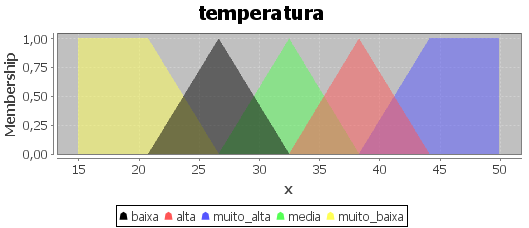
\includegraphics[width=1\linewidth]{fuzzy_temperatura}
  \caption{Função de pertinência da variável \textit{temperatura}.}
  \label{fig:fuzzytemperatura}
\end{figure}

O artigo que forneceu os dados de base não disponibilizou diretamente os valores de temperatura usados para obter os resultados, por isso foi preciso usar engenharia reversa para poder chegar aos valores usados.
Para conseguir encontrar esses dados foram usados os valores de evapotranspiração fornecidos no artigo. Para usar esses dados foi pesquisado como esses valores eram calculados. Esse cálculo foi encontrado no site da Embrapa.
O cálculo de evapotranspiração da cultura se encontra na fórmula abaixo:

$$ 
  ET_c = K_c \times ET_o 
$$


A variável $K_c$ se refere ao estágio de desenvolvimento da plantação, no caso do artigo esse valor estava em 0.5. A variável $ET_o$ é a evapotranspiração de referência do cia, para ser realizado o cálculo dessa variável e para ela ser usada na fórmula acima é usada a seguinte fórmula:

$$
  ETo = 0,0135 \times K \times R_a \times (T_{max} - T_{min}) \times (T_{med} + 17,8)
$$

A variável $K$ é uma constante que possui o valor 0,162 para regiões continentais. A variável $R_a$ é a radiação da atmosfera, esse valor varia de acordo com a latitude.

Como o cálculo do $ET_o$ ainda precisava dos valores de temperatura máxima e mínima medidos no dia não foi possível chegar aos valores exatos que o artigo usou, então foram verificados valores aproximados para se fazer o cálculo do $ET_o$ e $ET_c$.

Verificando os valores aproximados nos cálculos foi possível chegar a possíveis valores para a temperatura medida nos dias em que os autores do artigo realizaram os testes do sistema. Esses valores puderam ser testados no sistema e foi percebido que os valores obtidos não ficaram muito abaixo dos dados apresentados no artigo base.

A variável \textit{umidade} se refere aos valores medidos de umidade do solo durante o dia. Esses valores são de grande importância para poder determinar o tempo necessário de irrigação. Estão ligados a variável \textit{umidade} os conjuntos \{\textit{muito baixa}, \textit{baixa}, \textit{média}, \textit{alta}, \textit{muito alta}\}. E podemos ver suas Função de Pertinência a seguir.

$$
  U_{muito~baixa} = \left\{
  \begin{array}{lll}
  1 & se & 0 \leqslant x \leqslant 35 \\
  \frac{44 - x}{44 - 35} & se & 35 \leqslant x \leqslant 44 \\
  0 & \multicolumn{2}{l}{caso~contrario}
  \end{array}
  \right.
$$

$$
  U_{baixa} = \left\{
  \begin{array}{lll}
  \frac{x - 35}{44 - 35} & se & 35 \leqslant x \leqslant 44 \\
  \frac{53 - x}{53 - 44} & se & 44 \leqslant x \leqslant 53 \\
  0 & \multicolumn{2}{l}{caso~contrario}
  \end{array}
  \right.
$$

$$
  U_{media} = \left\{
  \begin{array}{lll}
  \frac{x - 44}{53 - 44} & se & 44 \leqslant x \leqslant 53 \\
  \frac{62 - x}{62 - 53} & se & 53 \leqslant x \leqslant 62 \\
  0 & \multicolumn{2}{l}{caso~contrario}
  \end{array}
  \right.
$$

$$
  U_{alta} = \left\{
  \begin{array}{lll}
  \frac{x - 53}{62 - 53} & se & 53 \leqslant x \leqslant 62 \\
  \frac{71 - x}{71 - 62} & se & 62 \leqslant x \leqslant 71 \\
  0 & \multicolumn{2}{l}{caso~contrario}
  \end{array}
  \right.
$$

$$
  U_{muito~alta} = \left\{
  \begin{array}{lll}
  \frac{x - 62}{71 - 62} & se & 62 \leqslant x \leqslant 71 \\
  1 & se & 71 \leqslant x \leqslant 100 \\
  0 & \multicolumn{2}{l}{caso~contrario}
  \end{array}
  \right.
$$

A Figura~\ref{fig:fuzzyumidade} representa gráfico gerado pelas fórmulas anteriores para a variável \textit{umidade}.

\begin{figure}[H]
  \centering
  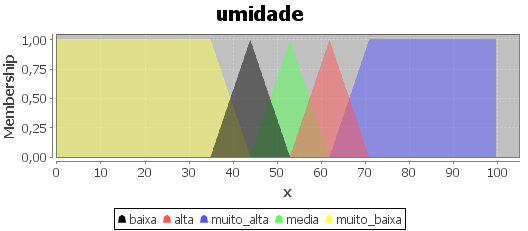
\includegraphics[width=1\linewidth]{fuzzy_umidade}
  \caption{Função de pertinência da variável \textit{umidade}.}
  \label{fig:fuzzyumidade}
\end{figure}

A variável \textit{estágio} se refere aos estágios de crescimento da plantação, o nível de água aumenta conforme o estágio de crescimento é mais avançado. Estão ligados a variável \textit{estágio} os conjuntos fuzzy \{\textit{crescimento}, \textit{desenvolvimento} e \textit{maturação}\}. E podemos ver suas Função de Pertinência a seguir.

$$
  E_{crescimento} = \left\{
  \begin{array}{lll}
  1 & se & 0 \leqslant x \leqslant 53 \\
  \frac{75 - x}{75 - 53} & se & 53 \leqslant x \leqslant 75 \\
  0 & \multicolumn{2}{l}{caso~contrario}
  \end{array}
  \right.
$$

$$
  E_{desenvolvimento} = \left\{
  \begin{array}{lll}
  \frac{x - 53}{75 - 53} & se & 53 \leqslant x \leqslant 75 \\
  \frac{98 - x}{98 - 75} & se & 75 \leqslant x \leqslant 98 \\
  0 & \multicolumn{2}{l}{caso~contrario}
  \end{array}
  \right.
$$

$$
  E_{maturacao} = \left\{
  \begin{array}{lll}
  \frac{x - 75}{98 - 75} & se & 75 \leqslant x \leqslant 98 \\
  1 & se & 98 \leqslant x \leqslant 100 \\
  0 & \multicolumn{2}{l}{caso~contrario}
  \end{array}
  \right.
$$

A Figura~\ref{fig:fuzzyestagio} representa gráfico gerado pelas fórmulas anteriores para a variável \textit{estagio}.

\begin{figure}[H]
  \centering
  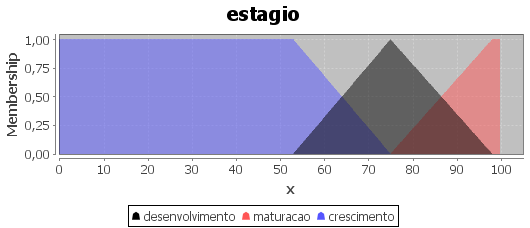
\includegraphics[width=1\linewidth]{fuzzy_estagio}
  \caption{Função de pertinência da variável \textit{estagio}.}
  \label{fig:fuzzyestagio}
\end{figure}

A umidade também não foi informada nos dados apresentados no artigo, então a umidade foi estimada tomando como base a temperatura. Visto que a região onde o sistema foi testado no artigo é uma região quente, foi estimado que a umidade ficava dentro de uma média de valores baixos.

A variável \textit{tempo} é a variável de saída do sistema, que indica o tempo que irá durar a irrigação da plantação. Estão ligados a variável \textit{tempo} os conjuntos \{\textit{muito curto}, \textit{curto}, \textit{médio}, \textit{longo} e \textit{muito longo}\}. E na Figura~\ref{fig:desfuzzytempo} podemos ver sua Função de Pertinência.

$$
  I_{muito~curto} = \left\{
  \begin{array}{lll}
  1 & se & 0 \leqslant x \leqslant 3.3 \\
  \frac{6.6 - x}{6.6 - 3.3} & se & 3.3 \leqslant x \leqslant 6.6 \\
  0 & \multicolumn{2}{l}{caso~contrario}
  \end{array}
  \right.
$$

$$
  I_{curto} = \left\{
  \begin{array}{lll}
  \frac{x - 3.3}{6.6 - 3.3} & se & 3.3 \leqslant x \leqslant 6.6 \\
  \frac{10 - x}{10 - 6.6} & se & 6.6 \leqslant x \leqslant 10 \\
  0 & \multicolumn{2}{l}{caso~contrario}
  \end{array}
  \right.
$$

$$
  I_{medio} = \left\{
  \begin{array}{lll}
  \frac{x - 6.6}{10 - 6.6} & se & 6.6 \leqslant x \leqslant 10 \\
  \frac{13.3 - x}{13.3 - 10} & se & 10 \leqslant x \leqslant 13.3 \\
  0 & \multicolumn{2}{l}{caso~contrario}
  \end{array}
  \right.
$$

$$
  I_{longo} = \left\{
  \begin{array}{lll}
  \frac{x - 10}{13.3 - 10} & se & 10 \leqslant x \leqslant 13.3 \\
  \frac{16.6 - x}{16.6 - 13.3} & se & 13.3 \leqslant x \leqslant 16.6 \\
  0 & \multicolumn{2}{l}{caso~contrario}
  \end{array}
  \right.
$$

$$
  I_{muito~longo} = \left\{
  \begin{array}{lll}
  \frac{x - 13.3}{16.6 - 13.3} & se & 13.3 \leqslant x \leqslant 16.6 \\
  1 & se & 16.6 \leqslant x \leqslant 20 \\
  0 & \multicolumn{2}{l}{caso~contrario}
  \end{array}
  \right.
$$

A Figura~\ref{fig:desfuzzytempo} representa gráfico gerado pelas fórmulas anteriores para a variável \textit{tempo}.

\begin{figure}[H]
  \centering
  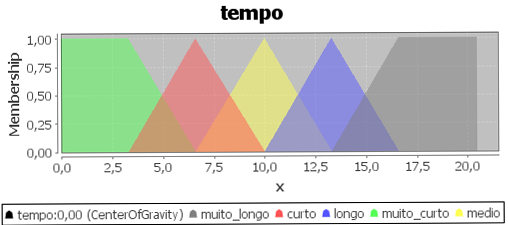
\includegraphics[width=1\linewidth]{desfuzzy_tempo}
  \caption{Função de pertinência da variável \textit{tempo}.}
  \label{fig:desfuzzytempo}
\end{figure}

%\vfill 
%\columnbreak

\section{Base de Regras}

O sistema possui um conjunto de 75 regras para controlar o sistema de irrigação. Esse conjunto é subdividido em 3 conjuntos, cada um desses conjuntos se refere a um estágio do crescimento da plantação.

Os 3 subconjuntos possuem a mesma combinação de regras referentes a temperatura e umidade do solo, diferenciando apenas com respeito ao tempo de irrigação, que é mais influenciado pelo estágio da plantação em cada subconjunto.

A seguir são apresentadas as bases de regras de todos os 3 subconjuntos. Nas bases de regras presentes nas Tabelas~\ref{tab:RegrasCrescimento},~\ref{tab:RegrasDesenvolvimento}~e~\ref{tab:RegrasMaturacao} é possível observar como o estágio de \textit{crescimento} da plantação influencia o tempo de irrigação, seguido da combinação da \textit{temperatura} e da \textit{umidade} do solo:

\end{multicols}


% CRESCIMENTO

\begin{table}[h]
  \centering
  \begin{tabular}{|c|c|c|c|c|c|c|}
    \hline 
    \multicolumn{2}{|c|}{\multirow{2}{*}{\textbf{Estágio de \textit{crescimento}}}}  &  \multicolumn{5}{c|}{\textbf{Temperatura}} \\ 
    \cline{3-7}
     \multicolumn{2}{|c|}{}  & \textbf{muito baixa} & \textbf{baixa} & \textbf{média} & \textbf{alta} & \textbf{muito alta} \\ 
    \hline 
    \multirow{5}{*}{\textbf{\rotatebox[origin=c]{90}{Umidade}}} & \textbf{muito baixa} 
                          & curto & médio & longo & longo & muito longo \\ 
    \cline{2-7}
    & \textbf{baixa}      & médio & médio & médio & médio & longo \\ 
    \cline{2-7}
    & \textbf{média}      & curto & curto & curto & curto & médio \\ 
    \cline{2-7}
    & \textbf{alta}       & muito curto & muito curto & muito curto & muito curto & muito curto \\ 
    \cline{2-7}
    & \textbf{muito alta} & muito curto & muito curto & muito curto & muito curto & muito curto \\ 
    \hline 
  \end{tabular} 
  
  \caption{Base de regras quando estagio em \textit{crescimento}.}
  \label{tab:RegrasCrescimento}
  \vspace{-0.5cm}
\end{table}


% DESENVOLVIMENTO
\begin{table}[h]
\centering
\begin{tabular}{|c|c|c|c|c|c|c|}
  \hline 
  \multicolumn{2}{|c|}{\multirow{2}{*}{\textbf{Estágio de \textit{desenvolvimento}}}}  &  \multicolumn{5}{c|}{\textbf{Temperatura}} \\ 
  \cline{3-7}
  \multicolumn{2}{|c|}{}  & \textbf{muito baixa} & \textbf{baixa} & \textbf{média} & \textbf{alta} & \textbf{muito alta} \\ 
  \hline 
  \multirow{5}{*}{\textbf{\rotatebox[origin=c]{90}{Umidade}}} & \textbf{muito baixa} 
                        & médio & médio & longo & longo & muito longo \\ 
  \cline{2-7}
  & \textbf{baixa}      & médio & médio & médio & longo & muito longo \\ 
  \cline{2-7}
  & \textbf{média}      & curto & curto & curto & médio & longo \\ 
  \cline{2-7}
  & \textbf{alta}       & muito curto & muito curto & curto & curto & longo \\ 
  \cline{2-7}
  & \textbf{muito alta} & muito curto & muito curto & muito curto & curto & médio \\ 
  \hline 
\end{tabular} 

\caption{Base de regras quando estagio em \textit{desenvolvimento}.}
\label{tab:RegrasDesenvolvimento}
\vspace{-0.5cm}
\end{table}


% MATURAÇÂO
\begin{table}[h]
\centering
\begin{tabular}{|c|c|c|c|c|c|c|}
  \hline 
  \multicolumn{2}{|c|}{\multirow{2}{*}{\textbf{Estágio de \textit{maturação}}}}  &  \multicolumn{5}{c|}{\textbf{Temperatura}} \\ 
  \cline{3-7}
  \multicolumn{2}{|c|}{}  & \textbf{muito baixa} & \textbf{baixa} & \textbf{média} & \textbf{alta} & \textbf{muito alta} \\ 
  \hline 
  \multirow{5}{*}{\textbf{\rotatebox[origin=c]{90}{Umidade}}} & \textbf{muito baixa} 
                        & médio & médio & longo & longo & muito longo \\ 
  \cline{2-7}
  & \textbf{baixa}      & médio & médio & médio & longo & muito longo \\ 
  \cline{2-7}
  & \textbf{média}      & médio & médio & médio & longo & muito longo \\ 
  \cline{2-7}
  & \textbf{alta}       & curto & curto & curto & médio & longo \\ 
  \cline{2-7}
  & \textbf{muito alta} & muito curto & curto & curto & curto & médio \\ 
  \hline 
\end{tabular} 

\caption{Base de regras quando estagio em \textit{maturação}.}
\label{tab:RegrasMaturacao}
\vspace{-0.5cm}
\end{table}


\begin{multicols}{2}
  
Por meio das combinações de temperatura, umidade do solo e estágio do crescimento da plantação é possível verificar qual é a quantidade de tempo mais ideal para se irrigar a plantação. Com base nessas regras o sistema é capaz de usar os valores de entrada e irrigar apenas o tempo que realmente é necessário, sem desperdiçar água.


\subsection{Definições de Funcionamento do Sistema de Inferência}

As T-normas são funções de pertinência que possuem determinadas características, como:

~

~

\vfill
\columnbreak

\begin{itemize}
  \item Limite e condição de contorno: $\mu(x,0) = x, \mu(x,1) = 1$
  \item Comutatividade: $\mu(x,y) = \mu(y,x)$
  \item Associatividade: $\mu(\mu(x,y),z) = \mu(x, \mu(y,z)) $
  \item Monotonicidade: Se $x \leq x\textquoteright$ e $y \leq y\textquoteright$ então $\mu(x,y) \leq \mu( x\textquoteright ,y\textquoteright )$
\end{itemize}


O conectivo \textit{E} é uma T-norma, pois ele atende a todos os parâmetros listados acima. Ele pode ser formado por diferentes formas de T-normas. A mais usada é a T-norma de Zadeh. Essa T-norma usa a função \textit{mínimo} para poder fazer a intersecção de dois conjuntos fuzzy.

O conectivo \textit{E} que foi usado para fazer as regras de inferência no desenvolvimento do trabalho usou a T-norma de Zadeh, pois ao se combinar diferentes valores de umidade e temperatura o mais apropriado era usar o valor mínimo entre eles para poder disparar as regras, dessa forma é mais provável atingir a quantidade de tempo necessária para irrigação sem causar desperdício.

Como existe um conjunto de três variáveis de entrada que são modeladas para conjuntos fuzzy é preciso analisar a junção desses dados para poder gerar o resultado da regra. Para fazer a ativação do consequente nas regras é usada a função mínimo, visto que é preciso unir os valores das três variáveis.

A função mínimo é a mais adequada para ser usada porque as regras são geradas usando a implicação de Mandani, onde é determinado que o valor do antecedente da regra não pode ser maior que o seu consequente, então deve ser usado o menor valor entre as variáveis para poder disparar o consequente da regra.

Então os três valores de entrada são atribuídos às regras e é verificado o menor valor entre as variáveis.

Para se fazer a acumulação das regras é usada a função de agregação \textit{máximo}. Essa função é usada porque diferentes regras podem ser ativadas com os mesmos valores das variáveis de entrada, então é preciso levar em consideração todos os valores das regras que foram ativadas.

Essa função faz a união dos valores para verificar o quanto a condição de cada regra é satisfeita, ela combina todos os resultados em um único conjunto fuzzy resultante formado pelos valores de saída das regras.

O método usado para a defuzzificação dos valores obtidos na agregação das regras foi o método do centro de gravidade.

Esse processo ocorre na interface de defuzzificação, onde o valor fuzzy resultante da agregação das regras é convertido para um valor crisp que melhor represente os resultados obtidos pelas demais fases do sistema.

O método do centro de área é um método de defuzzificação que analisa o conjunto fuzzy resultante da agregação dos resultados das regras de inferência. Nesse método é calculada a área do conjunto fuzzy e em qual ponto esse conjunto é dividido em duas partes com áreas iguais. Para achar o ponto onde dividir o conjunto ele realiza a média ponderada das regiões que formam o conjunto. Após realizar o cálculo da média ponderada é obtido um valor crisp que será a saída do sistema.


\section{Cenários e Análise dos Resultados}

O artigo que serviu como base para o trabalho se concentrou em um período que a plantação estava apenas no estágio de crescimento, então os dados usados se referem apenas a esse cenário. As regras referentes aos outros estágios foram feitas, mas os testes não puderam ser realizados com dados reais.

Nesta seção são apresentadas diferentes formas de execução do sistema de controle fuzzy, mostrando situações que comprovam que a implementação do projeto conseguiu simular situações que ocorreriam em sistemas e situações reais.

Cada uma das diferentes situações a serem executadas no sistema fuzzy é denominada como um cenário.


\subsection{Cenário 1: Estágio de Crescimento}
O artigo~\cite{ceballos2015fuzzy} que foi usado como base para o desenvolvimento do trabalho se concentrou em um único estágio do desenvolvimento da plantação, sendo este o estágio inicial de crescimento. Então o artigo modelou apenas a base de regras para este estágio.

Para poder verificar diferentes tipos de cenário foi verificada a diferença de temperatura dentro dos dados fornecidos no artigo. Como todos os testes foram feitos no estágio de crescimento da plantação, o cenário se foca em uma plantação ainda nas fases iniciais de crescimento.

Os testes que foram feitos se encontram em uma faixa definida de umidade e temperatura. A umidade não variou para valores altos, enquanto a temperatura não variou para valores baixos.

A Figura~\ref{fig:densidadecrescimento} mostra os resultados de tempo obtidos em relação à temperatura e umidade em uma faixa de densidade. Quanto mais escuro, mais tempo de irrigação é necessário. O intervalo de temperatura e umidade estão indicados por pontos no gráfico.

\begin{figure}[H]
  \centering
  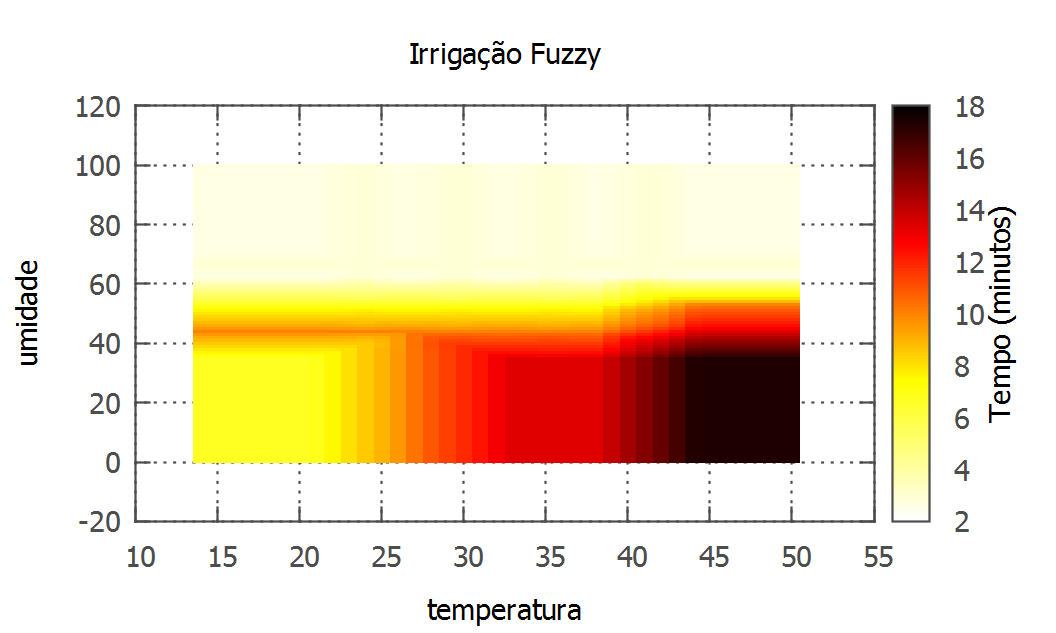
\includegraphics[width=1\linewidth]{densidade_crescimento}
  \caption{Gráfico de densidade do tempo de irrigação quando em estágio de \textit{crescimento}.}
  \label{fig:densidadecrescimento}
\end{figure}

\subsection{Cenário 2: Estágio de Desenvolvimento}
Os autores do artigo~\cite{ceballos2015fuzzy} não modelaram o sistema para os demais estágios de crescimento da plantação, porém foi possível modelar as regras para esses estágios se baseando no conjunto de regras criadas para o estágio de crescimento.

Os testes no cenário onde a plantação se encontrava no estágio de desenvolvimento foram feitos usando os mesmos valores que no cenário onde a plantação estava no estágio de crescimento, apenas foi alterada a informação sobre o estágio em que a plantação se encontrava.

A Figura~\ref{fig:densidadematuracao} mostra os resultados obtidos para o tempo de irrigação em relação a temperatura e umidade:

\begin{figure}[H]
  \centering
  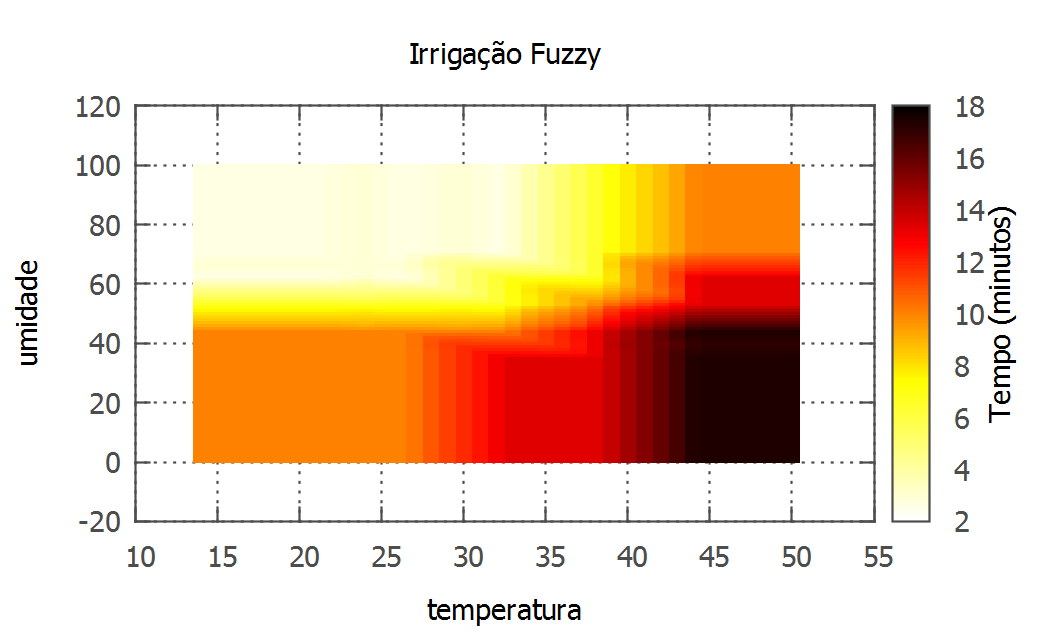
\includegraphics[width=1\linewidth]{densidade_desenvolvimento}
  \caption{Gráfico de densidade do tempo de irrigação quando em estágio de \textit{desenvolvimento}.}
  \label{fig:densidadedesenvolvimento}
\end{figure}

%\vfill
\columnbreak

\subsection{Cenário 3: Estágio de Maturação}

No artigo~\cite{ceballos2015fuzzy}, também não foi feita uma modelagem para o estágio de maturação da plantação, então o conjunto de regras também foi deduzido com base no conjunto usado para o estágio de crescimento.

Os testes nesse cenário também foram feitos usando os dados fornecidos pelo artigo, mudando apenas os valores com respeito ao estágio de crescimento da plantação.

Os resultados obtidos para o tempo de irrigação se encontram na Figura~\ref{fig:densidadematuracao}.

\begin{figure}[H]
  \centering
  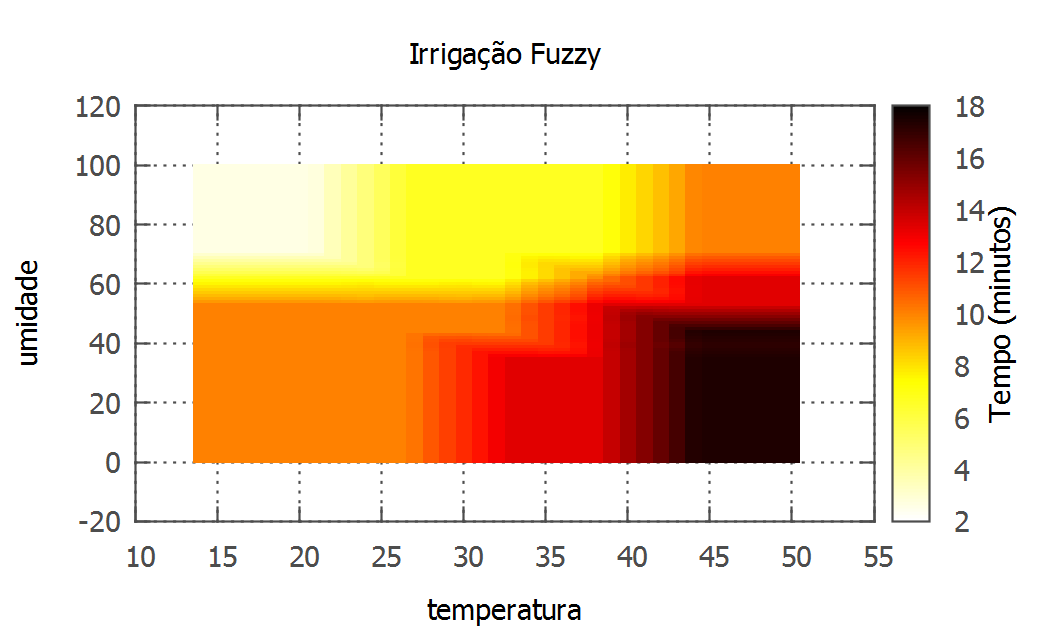
\includegraphics[width=1\linewidth]{densidade_maturacao}
  \caption{Gráfico de densidade do tempo de irrigação quando em estágio de \textit{maturação}.}
  \label{fig:densidadematuracao}
\end{figure}

%\vfill
%\columnbreak

\end{multicols}

\pagebreak

\begin{multicols}{2}

\section*{Conclusão}
\addcontentsline{toc}{section}{Conclusão}
Um sistema de irrigação é crucial para o cultivo de qualquer tipo de planta, mas um processo manual já não é algo mais viável e não existe um controle do gasto dessa forma, por isso existem muitos sistemas de irrigação automáticos. Esses sistemas facilitam o trabalho de agricultores, mas eles ainda não chegam ao uso eficiente de água, pois eles não analisam o quanto de água a plantação precisa, apenas distribuem a quantidade de água que foi programada.

A lógica fuzzy permite que sistemas sejam feitos com valores mais próximos da realidade, então um sistema de irrigação fuzzy iria permitir um gerenciamento melhor da água para irrigar a plantação, pois não seria despejada sempre a mesma quantidade de água, mas sim a quantidade realmente necessária.

Com base na temperatura, umidade do solo e estágio de desenvolvimento da plantação foi montado um conjunto de regras que iria indicar o tempo necessário para irrigar a plantação. Esse conjunto de regras foi montado com base nos conjuntos fuzzy criados para cada variável de entrada do sistema. Através desses valores é calculado o tempo necessário para o solo ser irrigado a quantidade suficiente.

Devido aos problemas para se obter os dados corretos não foi possível constatar que o sistema chegou aos mesmo resultados que o artigo que serviu de base para o trabalho, porém os resultados se mostraram satisfatórios, visto que a saída do sistema não ficou muito abaixo das saídas registradas pelos autores do artigo. Também foi possível modelar as demais regras que os autores não fizeram por não terem testado o sistema com plantações em outros estágios de crescimento. Com base nos dados iniciais foi possível testar valores aproximados para os demais estágios e os resultados pareceram adequados.

Com base nesses resultados é possível afirmar que o sistema usando lógica fuzzy para automatizar a irrigação de plantações é uma opção a ser considerada. Para trabalhos futuros seria interessante analisar o sistema com dados de outras plantações e em diferentes estágios e também ter uma base de dados para saber qual a quantidade de água necessária para a plantação de teste. Dessa forma será possível constatar de forma precisa se o sistema é eficaz, sem ser necessário fazer aproximações e por fazer ajustes nas regras, caso seja necessário.

\end{multicols}

%\begin{multicols}{2}
% ---
% Finaliza a parte no bookmark do PDF, para que se inicie o bookmark na raiz
% ---
\bookmarksetup{startatroot}% 
% ---



% ----------------------------------------------------------
% ELEMENTOS PÓS-TEXTUAIS
% ----------------------------------------------------------
\postextual

% ----------------------------------------------------------
% Referências bibliográficas
% ----------------------------------------------------------
\bibliography{Sistema_de_Irrigacao_Fuzzy}

\end{document}
